\documentclass[12pt]{article}
\usepackage{lingmacros}
\usepackage{tree-dvips}
\usepackage{amsmath,amssymb}
\usepackage{tabularx}
\usepackage{graphicx}
\usepackage[a4paper, total={6in, 8in}]{geometry}
\DeclareMathOperator*{\argmax}{argmax}


\begin{document}

\begin{titlepage}
    \begin{center}
        \vspace*{1cm}
         \textbf{\huge Statistical structured prediction} \\        
        \vspace{0.25cm}
         {\LARGE Question set (Part II)}\\
        \vfill
        Adrián Vázquez Barrera \\
        \vspace{0.25cm}
        Polytechnic University of Valencia\\
        \vspace{0.25cm}
        \textbf{January 2022}
             
    \end{center}
 \end{titlepage}

\newpage

\section*{Pregunta 1 (2 puntos)}
Explique brevemente las diferencias entre la clasificación y la predicción estructurada de resultados. Cite dos ejemplos de aplicación de cada paradigma.
\\\\
Los problemas de clasificación se fundamentan en catalogar una serie de muestras en un conjunto acotado de clases $C$. 
De esta forma, este problema puede formularse probabilísticamente determinando
una clase $c^* \in {1,2,...,C}$, cuya probabilidad
condicional dado el dato $x, P(c|x)$, sea máxima.
\\
\begin{equation*}
    c^* = \underset{c \in C}{\operatorname{argmax}} ~ P(c|x)
\end{equation*}
\\
La diferencia fundamental entre un problema de clasificación y un problema de predicción estructurada es que estos últimos poseen un espacio de hipótesis potencialmente infinito. Sobre todo porque las variables de salida $c^*$ son estructuradas, es decir, dependientes entre sí y siguiendo determinadas reglas.
\\\\
Los ejemplos típicos de tareas de clasificación suelen ser: reconocimiento de dígitos manuscritos aislados o categorización de mensajes de correo no deseado/legítimos. Por otra parte, utilizando técnicas de predicción estructurada se pueden resolver problemas como: síntesis de voz, transcripción de texto manuscrito, traducción automática o extraer información sintáctica de una frase.
\newpage
\section*{Pregunta 2 (2 puntos)}
Justifique por qué la descomposición Naive Bayes de la Ec.(5) es adecuada para el problema de reconocimiento de cariotipos.
\\\\
Partimos de la Eq.(4) que establece que, para toda secuencia de cromosomas inválidos su probabiliad es cero y $ \frac{1}{22!} $ en otro caso:
\\

\begin{equation*}
    P(x|h) =  
    \begin{cases}
        \frac{1}{22!} &\quad\text{if} ~ h_i \neq h_j \forall i \neq j, 1 \leq i, j \leq 22 \\
        \text{0} &\quad\text{otherwise} \\ 
      \end{cases}
\end{equation*}
\\
Por lo cual se considera que, la hipótesis de cada cromosoma es independiente de su posición con respecto al resto de la secuencia. Al asumir probabiliad cero para secuencias inválidas, se puede evaluar una elevada cantidad de parámetros sin que el coste computacional se dispare al utilizar modelos más simples:
\\
\begin{equation*}
    P(x|h) = P(x_1, ... , x_{22} | h_1, ... h_{22}) = 
\end{equation*}
\begin{equation*}
     P(x_1 | h_1) P(x_2 | h_1, h_2) P(x_3 | h_1, h_2, h_3)~...~P(x_{22} | h_1, h_2, h_3,~...~, h_{22})
\end{equation*}
\begin{equation*}
    \approx \prod_{i=1}^{22}{P(x_i|h_i)} 
\end{equation*}

\newpage

\section*{Pregunta 3 (2 puntos)}
Explica brevemente todos los pasos y supuestos necesarios para obtener la Ec.(9) a partir de la Ec.(7).
\\\\
Se parte de la Eq.(7), planteada en la página 24 de las diapositivas "Fundamentals of Multimodal Interaction in Pattern Recognition" vistas en clase:
\begin{equation*}
    \hat{h} = \underset{h \in H}{\operatorname{argmax}} ~ P(h|x, h', f)
\end{equation*}
\\
Aplicando la regla de la probabiliad conjunta, esta ecuación puede reescribirse como:
\begin{equation*}
    \hat{h} = \underset{h \in H}{\operatorname{argmax}} ~ \frac{P(h, x, h', f)}{P(x, h', f)}
\end{equation*}
\\
Como el denominador no depende de h, que es el parámetro a optimizar y del que depende el argmax, puede omitirse sin afectar al resultado:
\begin{equation*}
    \hat{h} = \underset{h \in H}{\operatorname{argmax}} ~ P(h, x, h', f)
\end{equation*}
\\
Aplicando la regla de la cadena  junto a la función $d = d(f)$ de decodificación, obtenemos: 
\begin{equation*}
    \hat{h} = \underset{h \in H}{\operatorname{argmax}} ~ P(d) \cdot P(h'|d) \cdot P(h|h', d) \cdot P(x | h', d ,h)
\end{equation*}
\\
Se descartan $P(d)$ y $P(h'| d)$ al no afectar en el cálculo del parámetro que se trata de maximizar:
\begin{equation*}
    \hat{h} = \underset{h \in H}{\operatorname{argmax}} ~ P(x | h', d ,h) \cdot P(h|h', d)
\end{equation*}
\\
Para terminar, sabemos que $h$ se obtiene a partir de $h'$ y $d$, por tanto la expresión $P(x | h’, d, h)$ puede simplificarse como $P(x | h)$. 
Esto lo conocemos a partir de la red bayesiana que modela las dependencias existentes entre las variables del problema. 

\begin{center}
    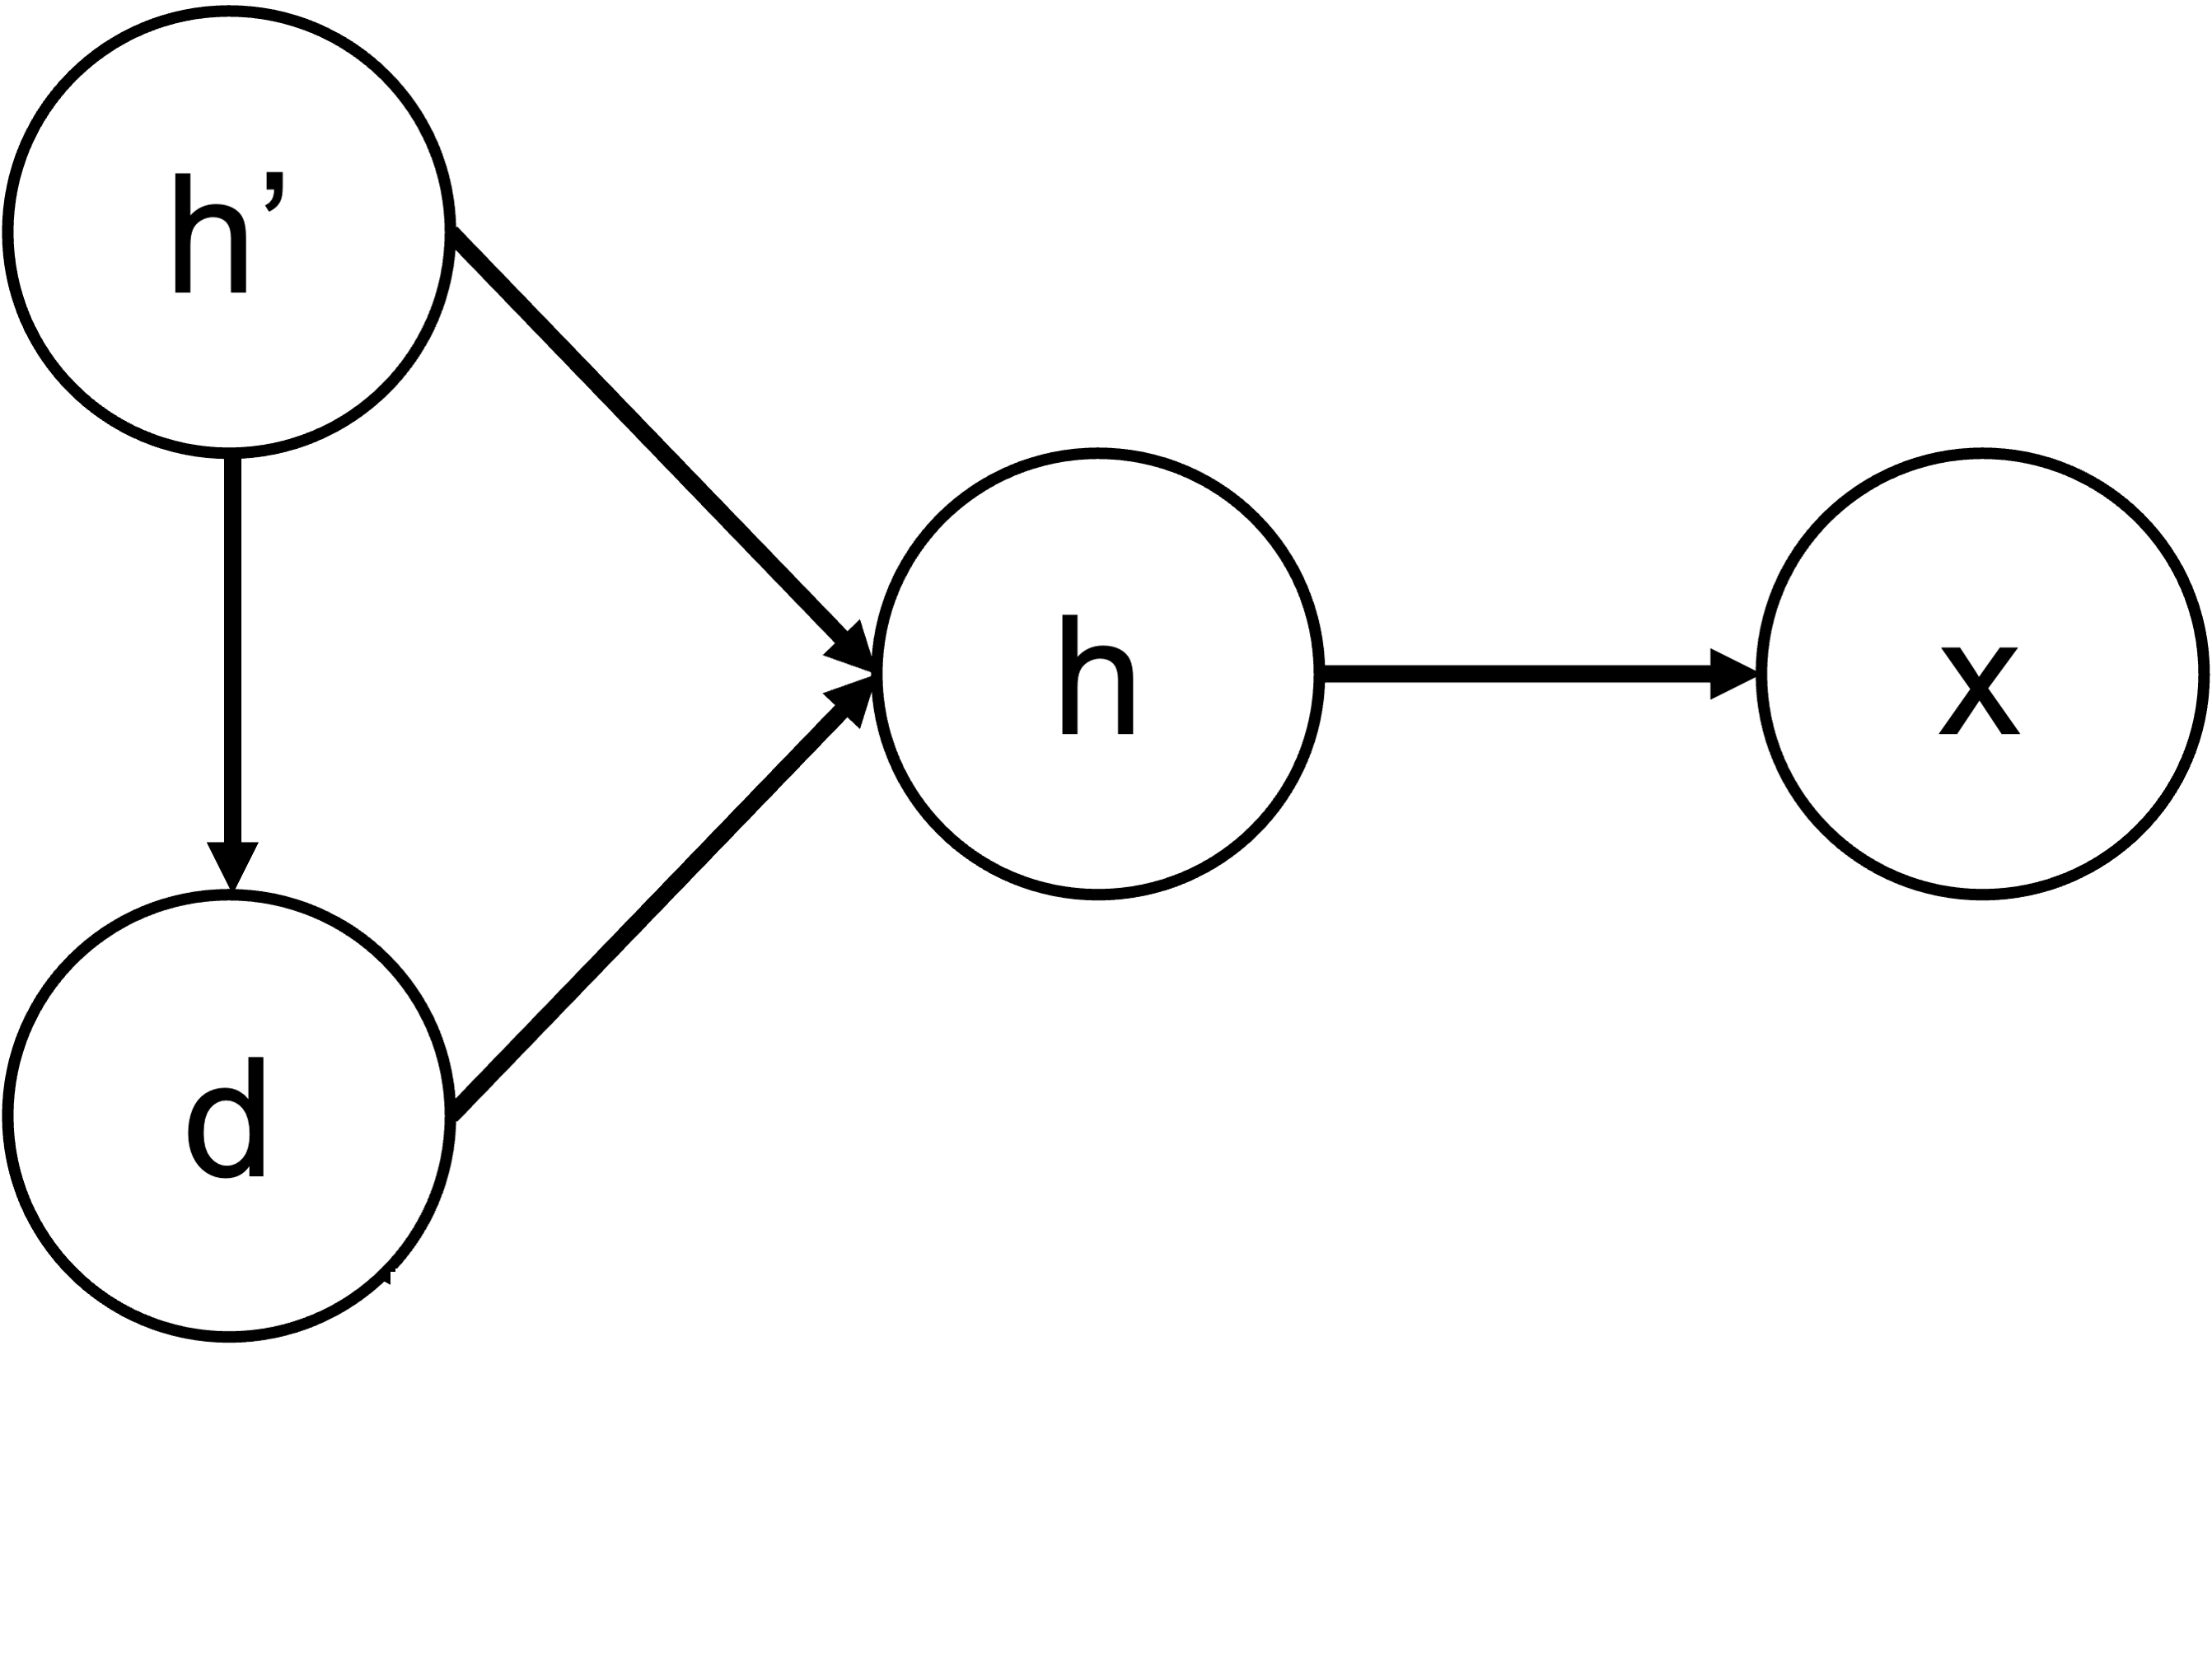
\includegraphics[width=0.25\columnwidth]{p2.png}
\end{center}
\begin{equation*}
    \hat{h} = \underset{h \in H}{\operatorname{argmax}} ~ P(x | h) \cdot P(h|h', d)
\end{equation*}

\newpage

\section*{Pregunta 6 (3 puntos)}
Explica brevemente todos los pasos y supuestos necesarios para derivar la Ec.(19) de la Ec.(7).
\\\\
Como se vio en el ejercicio anterior, partimos de la ecuación:
\begin{equation*}
    \hat{h} = \underset{h \in H}{\operatorname{argmax}} ~ P(h|x, h', f)
\end{equation*}
\\
De nuevo, aplicamos la regla conjunta:
\begin{equation*}
    \hat{h} = \underset{h \in H}{\operatorname{argmax}} ~ \frac{P(h, x, h', f)}{P(x, h', f)}
\end{equation*}
\\
Como el denominador no depende de h, que es el parámetro a optimizar y del que depende el argmax, puede omitirse sin afectar al resultado:
\begin{equation*}
    \hat{h} = \underset{h \in H}{\operatorname{argmax}} ~ P(h, x, h', f)
\end{equation*}
\\
Se incluye explícitamente toda posible descodificación de $f$ haciendo uso de la regla de la suma.
\\
\begin{equation*}
    \hat{h} = \underset{h \in H}{\operatorname{argmax}} ~ \sum_{d\in \mathcal{D} }{P(h, x, h', d, f)}
\end{equation*}
\\
Desarrollamos la ecuación aplicando la regla de la cadena:
\begin{equation*}
    \hat{h} = \underset{h \in H}{\operatorname{argmax}} ~ \sum_{d\in \mathcal{D} }{P(h') \cdot P(d|h') \cdot P(f|d) \cdot P(h|h', d) \cdot P(x|h) }
\end{equation*}
\\
Omitimos aquellos elementos que no dependen de $h$ para simplificar y sacamos factor común $P(x|h)$: 
\begin{equation*}
    \hat{h} = \underset{h \in H}{\operatorname{argmax}} ~ P(x|h) ~ \sum_{d\in \mathcal{D} }{P(d|h') \cdot P(f|d) \cdot P(h|h', d)}
\end{equation*}
\\
Aproximamos la suma por la moda, con esto podemos calcular más rápidamente la mejor hipótesis a expensas de perder precisión en el cálculo:
\begin{equation*}
    (\hat{h}, \hat{d}) \approx \underset{h, d}{\operatorname{argmax}} ~ P(x|h) \cdot {P(d|h') \cdot P(f|d) \cdot P(h|h', d)}
\end{equation*}

\newpage

\section*{Pregunta 7 (3 puntos)}
Explique brevemente bajo qué condiciones la solución dada por la Ec.(22-23) puede ser óptima. ¿Son válidas las mismas condiciones para la optimalidad de la solución dada por la Ec.(20-21)? ¿Por qué? Utilice el ejemplo del cariotipo para ilustrar sus respuestas.
\\\\
Las ecuaciones 22 y 23 serán óptimas si el tamaño del problema es igual a la cantidad de las $n$ decodificaciones más probables. Para el problema del cariotipo, las ecuaciones serán óptimas siempre que $n = 22$. Esto se debe a que las $22$ decodificaciones más probables contendrán toda la información necesaria para corregir los errores, lo que permitirá calcular la solución óptima.
\\\\
De las ecuaciones 20 y 21 no se puede decir lo mismo, esto es debido a que primero se obtiene una decodificación para el feedback que maximice $d$ que, una vez fijado se utiliza para obtener una hipótesis considerada óptima. Esta decodificación e hipótesis pueden unirse en múltiples combinaciones sub-óptimas y el número de estas excede el tamaño del problema. Por lo tanto, para un tamaño de problema igual a $n$ no se garantiza encontrar la hipótesis óptima.
\newpage

\section*{Pregunta 8 (3 puntos)}
Explique brevemente los conceptos y las principales diferencias entre los protocolos de interacción activa y pasiva
\\\\
Un protocolo de interacción activo se basa en delegar la supervisión de las hipótesis que deben ser revisadas al sistema. Por tanto, este debe otorgar una medida de confianza para cada hipótesis. De esa manera, el usuario podrá supervisar aquellas que muestren los peores resultados, ahorrando el trabajo de verificar manualmente todas las muestras. No obstante, con este protocolo, la calidad de los resultados dependerá en su mayoría de la calidad del propio sistema.
\\\\
Por otro lado, en el protocolo de interacción pasivo, es un usuario experto quien decide que muestras necesitan ser supervisadas. Esto significa comprobar todas y cada una de ellas, por lo que cabe asumir que, a su criterio, el sistema será perfecto.
\\\\
Existen dos formas de revisar las hipótesis del sistema:

\begin{itemize}
    \item Left-to-right: En la que se revisan las hipótesis siguiendo un orden establecido.
    \item Desultory: Revisando las hipótesis aleatoriamente.
  \end{itemize}

\end{document}

